%-------------------------------------------------------------------------------
% seq66_meta_events
%-------------------------------------------------------------------------------
%
% \file        seq66_meta_events.tex
% \library     Documents
% \author      Chris Ahlstrom
% \date        2017-07-23
% \update      2017-10-28
% \version     $Revision$
% \license     $XPC_GPL_LICENSE$
%
%     Provides a discussion of the MIDI GUI meta_events that Sequencer66
%     supports.
%
%-------------------------------------------------------------------------------

\section{Sequencer66 Meta Event / SysEx Support}
\label{sec:meta_events}

   \textsl{Sequencer66} attempts better support
   for MIDI Meta and System Exclusive events and a Tempo track.
   It supports the display of Set Tempo and Time Signature events.
   They can also be added and edited, in
   various ways.  For example, see \sectionref{sec:seq66_event_editor}.
   Only the first Time Signature event is used to modify playback.
   System Exclusive support is also still in progress, but very incomplete.
   This section consolidates the description of the meta-event support.
   The following topics apply:

   \begin{enumerate}
      \item Tempo display min/max in "usr" settings.
      \item Tempo display in main window.
      \item Tempo display in pattern editor.
      \item Tempo display in song editor.
      \item Tempo and Time signature display and editing in the event editor.
   \end{enumerate}

   First, we need to note \textsl{how} the tempo track is
   implemented in \textsl{Sequencer66}.  Rather than make a SeqSpec track for
   the tempo events, we use the MIDI specification mandate that
   Tempo events should occur only in the first track.
   \textsl{Sequencer66} treats Set Tempo and Time Signature as full-fledged
   MIDI events that can be viewed (and later, edited) in the existing
   user-interface.  Notes and other events can occur in the same
   track.
%  To reiterate, track 1 (pattern 0) is the only track where tempo events
%  can be placed and edited.

\subsection{"usr" BPM Display Settings}
\label{subsec:meta_events_usr}

   \textsl{Sequencer66} allows the tempo to range from 1 to 600 BPM
   (beats per minute).
   This range is hardwired into the application.
   To display tempo with a little more granularity,
   \textsl{Sequencer66} provides scaling for the tempo
   displays.  These values are found in the "usr" file:

   \begin{verbatim}
		0         # midi_bpm_minimum
		360       # midi_bpm_maximum
   \end{verbatim}

   See \sectionref{subsec:seq66_usr_file_user_midi_settings}, for more
   information.  This setting can only be made by editing the "usr" file
   while \textsl{Sequencer66} is not running.
   Note that this setting affects the global BPM setting ("c\_bpmtag").

% DO THESE SETTINGS apply to the global BPM or the tempo-track BPM???

\subsection{Composite Display of Tempos}
\label{subsec:meta_events_composite_display}

The following figure shows a composite picture of the various representations
of Set Tempo events.

\begin{figure}[H]
   \centering 
%  \includegraphics[scale=0.65]{meta/combined_tempo_display.png}
   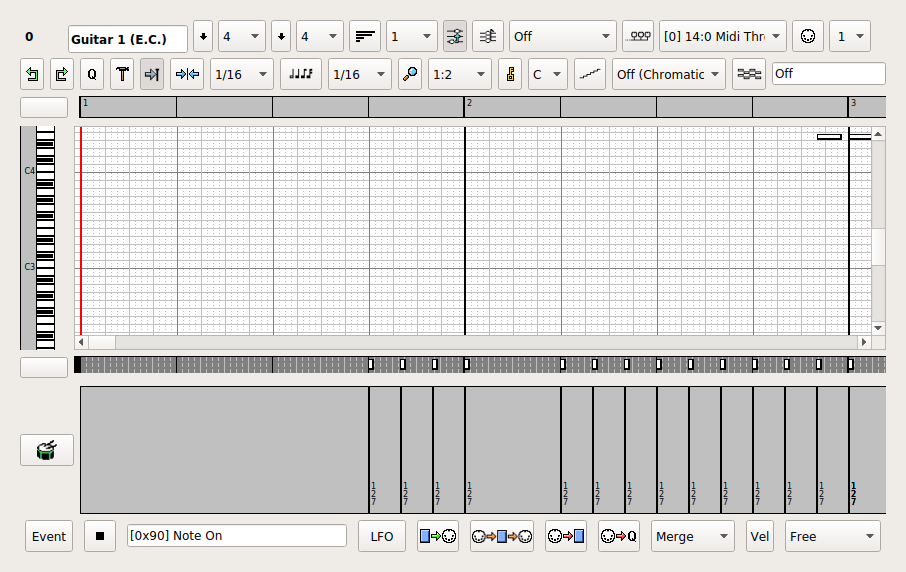
\includegraphics[scale=0.65]{roll.png}
   \caption{Various Tempo Displays}
   \label{fig:meta_events_tempo_displays}
\end{figure}

The \textsl{top} of the figure shows the magenta tempo lines in a pattern slot
that is currently being edited.  This view edited, but the
event editor and the main window's BPM settings can be used to add, delete, or
adjust the tempo.
The \textsl{middle} panel shows the very similar representation of the tempo in
the song editor.  This view does not allow editing of the tempo events.
The \textsl{bottom} shows tempo as an event (in the event strip) and a data
value in the data pane.  A tempo event can be added here by holding the Ctrl
key and painting an event in the event strip, and it can then be modified by
same method that note velocities can be edited.  Tempo events are
\textsl{always} shown in the event strip and the data pane, no matter what
other \textbf{Event} type has been selected.

\subsection{Tempo in the Main Window}
\label{subsec:meta_events_mainwid}

% The following figure shows a note and some tempo changes.
%
% \begin{figure}[H]
%   \centering 
%   \includegraphics[scale=1.0]{meta/mainwid_pattern_tempo.png}
%   \caption{Tempo in Pattern Slot}
%   \label{fig:meta_events_mainwid_slot}
% \end{figure}
%
% This figure is out-of-date.

The tempo is shown as a solid magenta-colored line at the relative height
for the tempo,
based on the minimum and maximum values configured in the "usr" file as
discussed above.
This pattern-slot tempo display is rudimentary.  It doesn't allow for ramping
of the tempo at present (except by recording while holding the BPM
spin-control), and cannot be directly edited in this window.
However, tempos can be logged or recorded via magenta-colored controls at the
bottom of the main window.

\begin{figure}[H]
   \centering 
%  \includegraphics[scale=0.75]{meta/tempo_recording.png}
   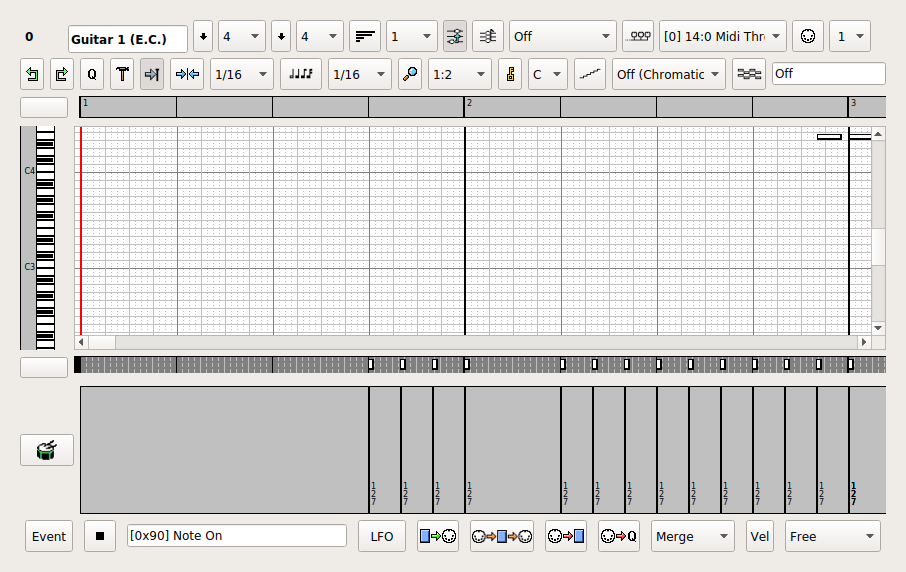
\includegraphics[scale=0.65]{roll.png}
   \caption{Tempo Recording Controls}
   \label{fig:meta_events_mainwid_tempo_recording}
\end{figure}

The 0th pattern slot shown in the figure is Track 1, the
MIDI Tempo track.  The magenta lines show the tempos already in that track.
Now look at the BPM control.  The first button to its right ("0") is the
tempo-tap button, used for setting a tempo by tapping in time to music.
The light-magenta button that comes next, when pressed while playback is
occurring, logs a tempo event at the current progress location and the
current BPM value in the BPM spin-field.  The dark magenta button to the right
of that toggles the mode of recording the changes to the BPM spin-button while
playback is occurring.
% (The "Q" button is for keep-queues, and is unrelated to
% tempo processing.)

Although pattern 0 might start out with a length of only a
measure or two, the timer continually ticks upward, and tempo events that
are recorded after the end of the track at still recorded, and
\textsl{they will extend the length of the tempo track}.
If the "show sequences key" option is enabled, the length of each track, in
measures, is shown at the top right of each main window pattern slot, so it can
be tracked by the user.

Once tempo events have been recorded, they can be tweaked (or deleted)
either in the pattern editor or in the event editor.  Generally, they are
treated like control events that are always available.  Deleting all tempo
events will not reduce the (possibly new) length of the sequence.
The Tempo track will \textsl{not} change tempo unless that track is unmuted.
This behavior is a feature, not a bug.

% \subsubsection{MIDI Metrics, PPQN}
% \label{subsubsec:meta_events_midi_ppqn}

%-------------------------------------------------------------------------------
% vim: ts=3 sw=3 et ft=tex
%-------------------------------------------------------------------------------
